\documentclass[conference]{IEEEtran}

\usepackage{cite}
\usepackage{amsmath,amssymb}
\usepackage{graphicx}
\usepackage{booktabs}
\usepackage{microtype}
\usepackage{url}

\graphicspath{{figures/}}
% Generated by scripts/build_paper_assets.py from results/*.json. Do not edit by hand.
\newcommand{\NumVariants}{8}
\newcommand{\NumExternal}{3}
\newcommand{\NumPolicies}{11}
\newcommand{\NumWorkloads}{6}
\newcommand{\NumCategories}{7}
\newcommand{\NumReplicates}{3}
\newcommand{\UnitsPerCell}{21}
\newcommand{\StepsPerRun}{9{,}000}
\newcommand{\TotalRuns}{1{,}386}
\newcommand{\TotalRunsRho}{1{,}386}
\newcommand{\BootB}{2{,}000}
\newcommand{\BankAurocMin}{0.925}
\newcommand{\BankAurocMax}{1.000}
\newcommand{\DefectMedianBelowHigh}{5}
\newcommand{\GlareMedianMin}{0.57}
\newcommand{\GoodPoolMin}{20}
\newcommand{\GoodPoolMax}{58}
\newcommand{\OpticalWorstCategory}{metal\_nut}
\newcommand{\OpticalWorstRate}{19.4\%}
\newcommand{\OpticalWorstTypes}{flip}
\newcommand{\OpticalNominalFlagMax}{0.0\%}
\newcommand{\NominalFABaseline}{4{,}616}
\newcommand{\NominalFABaselineLo}{1{,}557}
\newcommand{\NominalFABaselineHi}{8{,}374}
\newcommand{\NominalFAFull}{0.0}
\newcommand{\NominalFAEmaOnly}{40.6}
\newcommand{\NominalFABaselineZeroCats}{2}
\newcommand{\NominalFABaselineMaxCat}{metal\_nut}
\newcommand{\NominalFABaselineMaxCatVal}{14{,}780}
\newcommand{\GlarePerBurstBaseline}{2.63}
\newcommand{\GlarePerBurstBaselineLo}{2.24}
\newcommand{\GlarePerBurstBaselineHi}{3.14}
\newcommand{\AlertsPerEpisodeBaseline}{137.64}
\newcommand{\AlertsPerEpisodeBaselineLo}{125.15}
\newcommand{\AlertsPerEpisodeBaselineHi}{149.53}
\newcommand{\SustainedDelayBaseline}{0.1}
\newcommand{\MultiRecallBaseline}{0.78}
\newcommand{\CritFABaseline}{3{,}342}
\newcommand{\DegradedFABaseline}{4{,}253}
\newcommand{\StateFABaseline}{7{,}299}
\newcommand{\GlarePerBurstEmaKofn}{5.66}
\newcommand{\GlarePerBurstEmaKofnLo}{3.64}
\newcommand{\GlarePerBurstEmaKofnHi}{7.33}
\newcommand{\AlertsPerEpisodeEmaKofn}{153.95}
\newcommand{\AlertsPerEpisodeEmaKofnLo}{149.39}
\newcommand{\AlertsPerEpisodeEmaKofnHi}{157.89}
\newcommand{\SustainedDelayEmaKofn}{3.7}
\newcommand{\MultiRecallEmaKofn}{0.62}
\newcommand{\CritFAEmaKofn}{3{,}649}
\newcommand{\DegradedFAEmaKofn}{0.0}
\newcommand{\StateFAEmaKofn}{3{,}389}
\newcommand{\NominalFAEmaKofn}{0.0}
\newcommand{\GlarePerBurstFull}{0.66}
\newcommand{\GlarePerBurstFullLo}{0.44}
\newcommand{\GlarePerBurstFullHi}{0.83}
\newcommand{\AlertsPerEpisodeFull}{1.00}
\newcommand{\AlertsPerEpisodeFullLo}{1.00}
\newcommand{\AlertsPerEpisodeFullHi}{1.00}
\newcommand{\SustainedDelayFull}{3.7}
\newcommand{\MultiRecallFull}{1.00}
\newcommand{\CritFAFull}{4.0}
\newcommand{\DegradedFAFull}{120.9}
\newcommand{\StateFAFull}{1.3}
\newcommand{\GlarePerBurstTimer}{0.03}
\newcommand{\GlarePerBurstTimerLo}{0.01}
\newcommand{\GlarePerBurstTimerHi}{0.05}
\newcommand{\AlertsPerEpisodeTimer}{1.23}
\newcommand{\AlertsPerEpisodeTimerLo}{1.02}
\newcommand{\AlertsPerEpisodeTimerHi}{1.47}
\newcommand{\SustainedDelayTimer}{3.9}
\newcommand{\MultiRecallTimer}{0.61}
\newcommand{\CritFATimer}{104.2}
\newcommand{\DegradedFATimer}{5.1}
\newcommand{\StateFATimer}{107.0}
\newcommand{\NominalFATimer}{5.1}
\newcommand{\GlarePerBurstHyst}{0.59}
\newcommand{\GlarePerBurstHystLo}{0.35}
\newcommand{\GlarePerBurstHystHi}{0.86}
\newcommand{\AlertsPerEpisodeHyst}{1.58}
\newcommand{\AlertsPerEpisodeHystLo}{0.59}
\newcommand{\AlertsPerEpisodeHystHi}{2.93}
\newcommand{\SustainedDelayHyst}{0.4}
\newcommand{\MultiRecallHyst}{0.84}
\newcommand{\CritFAHyst}{125.1}
\newcommand{\DegradedFAHyst}{11.5}
\newcommand{\StateFAHyst}{105.5}
\newcommand{\NominalFAHyst}{3.4}
\newcommand{\GlarePerBurstFusion}{0.03}
\newcommand{\GlarePerBurstFusionLo}{0.01}
\newcommand{\GlarePerBurstFusionHi}{0.05}
\newcommand{\AlertsPerEpisodeFusion}{0.98}
\newcommand{\AlertsPerEpisodeFusionLo}{0.95}
\newcommand{\AlertsPerEpisodeFusionHi}{1.00}
\newcommand{\SustainedDelayFusion}{3.9}
\newcommand{\MultiRecallFusion}{1.00}
\newcommand{\CritFAFusion}{5.4}
\newcommand{\DegradedFAFusion}{30.7}
\newcommand{\StateFAFusion}{125.6}
\newcommand{\NominalFAFusion}{5.1}
\newcommand{\SustainedAlertsBaseline}{17{,}152}
\newcommand{\SustainedAlertsFull}{96}
\newcommand{\SustainedAlertReduction}{99.4\%}
\newcommand{\SustainedDelayFullMs}{122}
\newcommand{\MultiRecallNoFusion}{0.62}
\newcommand{\PerCatDelayMin}{3.0}
\newcommand{\PerCatDelayMax}{5.0}
\newcommand{\CritFAFullCI}{4.0}
\newcommand{\CritFAFullCILo}{1.3}
\newcommand{\CritFAFullCIHi}{6.8}
\newcommand{\CritFANoDiv}{117.0}
\newcommand{\StateFANoGating}{121.8}
\newcommand{\DegradedAlertsTotal}{314}
\newcommand{\DegradedOpticalAlerts}{147}
\newcommand{\DegradedSensorAlerts}{42}
\newcommand{\DegradedFAFullNoMaint}{26.9}
\newcommand{\EffFANomBaseline}{4{,}616}
\newcommand{\EffFANomBaselineLo}{1{,}557}
\newcommand{\EffFANomBaselineHi}{8{,}374}
\newcommand{\EffFANomBaselineWins}{5}
\newcommand{\EffFANomBaselineLosses}{0}
\newcommand{\EffFANomTimer}{5.1}
\newcommand{\EffFANomTimerLo}{0.0}
\newcommand{\EffFANomTimerHi}{15.4}
\newcommand{\EffFANomTimerWins}{1}
\newcommand{\EffFANomTimerLosses}{0}
\newcommand{\EffFANomHyst}{3.4}
\newcommand{\EffFANomHystLo}{0.0}
\newcommand{\EffFANomHystHi}{6.9}
\newcommand{\EffFANomHystWins}{2}
\newcommand{\EffFANomHystLosses}{0}
\newcommand{\EffFANomFusion}{5.1}
\newcommand{\EffFANomFusionLo}{0.0}
\newcommand{\EffFANomFusionHi}{15.4}
\newcommand{\EffFANomFusionWins}{1}
\newcommand{\EffFANomFusionLosses}{0}
\newcommand{\EffGlareBaseline}{1.97}
\newcommand{\EffGlareBaselineLo}{1.59}
\newcommand{\EffGlareBaselineHi}{2.44}
\newcommand{\EffGlareBaselineWins}{7}
\newcommand{\EffGlareBaselineLosses}{0}
\newcommand{\EffGlareTimer}{-0.64}
\newcommand{\EffGlareTimerLo}{-0.79}
\newcommand{\EffGlareTimerHi}{-0.42}
\newcommand{\EffGlareTimerWins}{0}
\newcommand{\EffGlareTimerLosses}{7}
\newcommand{\EffGlareHyst}{-0.07}
\newcommand{\EffGlareHystLo}{-0.32}
\newcommand{\EffGlareHystHi}{0.19}
\newcommand{\EffGlareHystWins}{3}
\newcommand{\EffGlareHystLosses}{4}
\newcommand{\EffGlareFusion}{-0.64}
\newcommand{\EffGlareFusionLo}{-0.79}
\newcommand{\EffGlareFusionHi}{-0.42}
\newcommand{\EffGlareFusionWins}{0}
\newcommand{\EffGlareFusionLosses}{7}
\newcommand{\EffAlertsEpBaseline}{136.64}
\newcommand{\EffAlertsEpBaselineLo}{124.15}
\newcommand{\EffAlertsEpBaselineHi}{148.53}
\newcommand{\EffAlertsEpBaselineWins}{7}
\newcommand{\EffAlertsEpBaselineLosses}{0}
\newcommand{\EffAlertsEpTimer}{0.23}
\newcommand{\EffAlertsEpTimerLo}{0.02}
\newcommand{\EffAlertsEpTimerHi}{0.47}
\newcommand{\EffAlertsEpTimerWins}{4}
\newcommand{\EffAlertsEpTimerLosses}{1}
\newcommand{\EffAlertsEpHyst}{0.58}
\newcommand{\EffAlertsEpHystLo}{-0.41}
\newcommand{\EffAlertsEpHystHi}{1.93}
\newcommand{\EffAlertsEpHystWins}{4}
\newcommand{\EffAlertsEpHystLosses}{3}
\newcommand{\EffAlertsEpFusion}{-0.02}
\newcommand{\EffAlertsEpFusionLo}{-0.05}
\newcommand{\EffAlertsEpFusionHi}{0.00}
\newcommand{\EffAlertsEpFusionWins}{0}
\newcommand{\EffAlertsEpFusionLosses}{1}
\newcommand{\EffDelayBaseline}{-3.6}
\newcommand{\EffDelayBaselineLo}{-4.0}
\newcommand{\EffDelayBaselineHi}{-3.2}
\newcommand{\EffDelayBaselineWins}{0}
\newcommand{\EffDelayBaselineLosses}{7}
\newcommand{\EffDelayTimer}{0.3}
\newcommand{\EffDelayTimerLo}{-0.4}
\newcommand{\EffDelayTimerHi}{1.0}
\newcommand{\EffDelayTimerWins}{3}
\newcommand{\EffDelayTimerLosses}{4}
\newcommand{\EffDelayHyst}{-3.3}
\newcommand{\EffDelayHystLo}{-3.5}
\newcommand{\EffDelayHystHi}{-3.1}
\newcommand{\EffDelayHystWins}{0}
\newcommand{\EffDelayHystLosses}{7}
\newcommand{\EffDelayFusion}{0.3}
\newcommand{\EffDelayFusionLo}{-0.4}
\newcommand{\EffDelayFusionHi}{1.0}
\newcommand{\EffDelayFusionWins}{3}
\newcommand{\EffDelayFusionLosses}{4}
\newcommand{\EffRecallMultiBaseline}{-0.22}
\newcommand{\EffRecallMultiBaselineLo}{-0.32}
\newcommand{\EffRecallMultiBaselineHi}{-0.12}
\newcommand{\EffRecallMultiBaselineWins}{6}
\newcommand{\EffRecallMultiBaselineLosses}{0}
\newcommand{\EffRecallMultiTimer}{-0.39}
\newcommand{\EffRecallMultiTimerLo}{-0.46}
\newcommand{\EffRecallMultiTimerHi}{-0.34}
\newcommand{\EffRecallMultiTimerWins}{7}
\newcommand{\EffRecallMultiTimerLosses}{0}
\newcommand{\EffRecallMultiHyst}{-0.16}
\newcommand{\EffRecallMultiHystLo}{-0.28}
\newcommand{\EffRecallMultiHystHi}{-0.05}
\newcommand{\EffRecallMultiHystWins}{5}
\newcommand{\EffRecallMultiHystLosses}{0}
\newcommand{\EffRecallMultiFusion}{0.00}
\newcommand{\EffRecallMultiFusionLo}{0.00}
\newcommand{\EffRecallMultiFusionHi}{0.00}
\newcommand{\EffRecallMultiFusionWins}{0}
\newcommand{\EffRecallMultiFusionLosses}{0}
\newcommand{\EffCritFAMultiBaseline}{3{,}338}
\newcommand{\EffCritFAMultiBaselineLo}{1{,}947}
\newcommand{\EffCritFAMultiBaselineHi}{4{,}585}
\newcommand{\EffCritFAMultiBaselineWins}{6}
\newcommand{\EffCritFAMultiBaselineLosses}{0}
\newcommand{\EffCritFAMultiTimer}{100.1}
\newcommand{\EffCritFAMultiTimerLo}{61.3}
\newcommand{\EffCritFAMultiTimerHi}{130.3}
\newcommand{\EffCritFAMultiTimerWins}{6}
\newcommand{\EffCritFAMultiTimerLosses}{0}
\newcommand{\EffCritFAMultiHyst}{121.1}
\newcommand{\EffCritFAMultiHystLo}{77.9}
\newcommand{\EffCritFAMultiHystHi}{150.2}
\newcommand{\EffCritFAMultiHystWins}{6}
\newcommand{\EffCritFAMultiHystLosses}{0}
\newcommand{\EffCritFAMultiFusion}{1.4}
\newcommand{\EffCritFAMultiFusionLo}{0.0}
\newcommand{\EffCritFAMultiFusionHi}{3.4}
\newcommand{\EffCritFAMultiFusionWins}{2}
\newcommand{\EffCritFAMultiFusionLosses}{0}
\newcommand{\EffFADegrBaseline}{4{,}132}
\newcommand{\EffFADegrBaselineLo}{1{,}288}
\newcommand{\EffFADegrBaselineHi}{7{,}592}
\newcommand{\EffFADegrBaselineWins}{5}
\newcommand{\EffFADegrBaselineLosses}{2}
\newcommand{\EffFADegrTimer}{-115.8}
\newcommand{\EffFADegrTimerLo}{-122.2}
\newcommand{\EffFADegrTimerHi}{-108.1}
\newcommand{\EffFADegrTimerWins}{0}
\newcommand{\EffFADegrTimerLosses}{7}
\newcommand{\EffFADegrHyst}{-109.4}
\newcommand{\EffFADegrHystLo}{-122.0}
\newcommand{\EffFADegrHystHi}{-89.1}
\newcommand{\EffFADegrHystWins}{0}
\newcommand{\EffFADegrHystLosses}{7}
\newcommand{\EffFADegrFusion}{-90.2}
\newcommand{\EffFADegrFusionLo}{-97.6}
\newcommand{\EffFADegrFusionHi}{-81.6}
\newcommand{\EffFADegrFusionWins}{0}
\newcommand{\EffFADegrFusionLosses}{7}
\newcommand{\EffFAStateBaseline}{7{,}298}
\newcommand{\EffFAStateBaselineLo}{4{,}322}
\newcommand{\EffFAStateBaselineHi}{10{,}961}
\newcommand{\EffFAStateBaselineWins}{7}
\newcommand{\EffFAStateBaselineLosses}{0}
\newcommand{\EffFAStateTimer}{105.8}
\newcommand{\EffFAStateTimerLo}{87.3}
\newcommand{\EffFAStateTimerHi}{126.4}
\newcommand{\EffFAStateTimerWins}{7}
\newcommand{\EffFAStateTimerLosses}{0}
\newcommand{\EffFAStateHyst}{104.2}
\newcommand{\EffFAStateHystLo}{63.1}
\newcommand{\EffFAStateHystHi}{140.1}
\newcommand{\EffFAStateHystWins}{6}
\newcommand{\EffFAStateHystLosses}{0}
\newcommand{\EffFAStateFusion}{124.4}
\newcommand{\EffFAStateFusionLo}{117.5}
\newcommand{\EffFAStateFusionHi}{134.4}
\newcommand{\EffFAStateFusionWins}{7}
\newcommand{\EffFAStateFusionLosses}{0}
\newcommand{\RhoNominalFABaseline}{4{,}615}
\newcommand{\RhoGlareBaseline}{2.60}
\newcommand{\RhoAlertsEpBaseline}{136.26}
\newcommand{\RhoDelayBaseline}{0.2}
\newcommand{\RhoCritFABaseline}{3{,}335}
\newcommand{\RhoRecallBaseline}{0.67}
\newcommand{\RhoNominalFAEmaKofn}{2{,}438}
\newcommand{\RhoGlareEmaKofn}{6.05}
\newcommand{\RhoAlertsEpEmaKofn}{146.19}
\newcommand{\RhoDelayEmaKofn}{3.7}
\newcommand{\RhoCritFAEmaKofn}{3{,}544}
\newcommand{\RhoRecallEmaKofn}{0.61}
\newcommand{\RhoNominalFAFull}{188.6}
\newcommand{\RhoGlareFull}{0.63}
\newcommand{\RhoAlertsEpFull}{1.07}
\newcommand{\RhoDelayFull}{3.7}
\newcommand{\RhoCritFAFull}{3.4}
\newcommand{\RhoRecallFull}{1.00}
\newcommand{\RhoNominalFATimer}{300.0}
\newcommand{\RhoGlareTimer}{0.06}
\newcommand{\RhoAlertsEpTimer}{1.58}
\newcommand{\RhoDelayTimer}{3.4}
\newcommand{\RhoCritFATimer}{111.6}
\newcommand{\RhoRecallTimer}{0.64}
\newcommand{\RhoNominalFAFusion}{300.0}
\newcommand{\RhoGlareFusion}{0.06}
\newcommand{\RhoAlertsEpFusion}{1.04}
\newcommand{\RhoDelayFusion}{3.4}
\newcommand{\RhoCritFAFusion}{21.4}
\newcommand{\RhoRecallFusion}{1.00}
\newcommand{\RhoNominalFAHyst}{105.1}
\newcommand{\RhoGlareHyst}{0.66}
\newcommand{\RhoAlertsEpHyst}{1.79}
\newcommand{\RhoDelayHyst}{0.7}
\newcommand{\RhoCritFAHyst}{116.3}
\newcommand{\RhoRecallHyst}{0.79}
\newcommand{\SensKLow}{2}
\newcommand{\SensKHigh}{6}
\newcommand{\SensCritKLow}{3.4}
\newcommand{\SensCritKHigh}{4.0}
\newcommand{\SensGlareKLow}{501}
\newcommand{\SensGlareKHigh}{159}
\newcommand{\SensDelayKLow}{1.6}
\newcommand{\SensDelayKHigh}{5.7}
\newcommand{\SensCritMin}{3.4}
\newcommand{\SensCritMax}{4.0}
\newcommand{\SensRecallMin}{1.00}
\newcommand{\SensCritDivLo}{4.0}
\newcommand{\SensCritDivHi}{4.0}
\newcommand{\SensGlareDivLo}{319}
\newcommand{\SensGlareDivHi}{319}
\newcommand{\SensCritAlphaLo}{4.0}
\newcommand{\SensCritAlphaHi}{3.4}
\newcommand{\SensGlareAlphaLo}{303}
\newcommand{\SensGlareAlphaHi}{261}
\newcommand{\SensCritCoolLo}{4.0}
\newcommand{\SensCritCoolHi}{3.4}
\newcommand{\SensGlareCoolLo}{319}
\newcommand{\SensGlareCoolHi}{239}
\newcommand{\GlareRateAssumed}{30}
\newcommand{\MuReviews}{60}
\newcommand{\LoadCrossFull}{40}
\newcommand{\LoadCrossEmaKofn}{0}
\newcommand{\LoadCrossTimer}{44}
\newcommand{\LoadCrossFusion}{55}
\newcommand{\LoadCrossBaseline}{0}
\newcommand{\PrecFullOneEp}{5\%}
\newcommand{\PrecTimerOneEp}{17\%}
\newcommand{\ShortK}{4}
\newcommand{\ShortN}{10}
\newcommand{\ShortRecallTarget}{0.95}
\newcommand{\ShortRecallBaselineOne}{0.96}
\newcommand{\ShortRecallBaselineTwo}{0.99}
\newcommand{\ShortRecallBaselineThree}{1.00}
\newcommand{\ShortRecallBaselineFive}{1.00}
\newcommand{\ShortRecallBaselineTen}{1.00}
\newcommand{\ShortMinLenBaseline}{1}
\newcommand{\ShortMinLenBaselineMs}{33}
\newcommand{\ShortRecallFullOne}{0.10}
\newcommand{\ShortRecallFullTwo}{0.43}
\newcommand{\ShortRecallFullThree}{0.70}
\newcommand{\ShortRecallFullFive}{0.91}
\newcommand{\ShortRecallFullTen}{0.99}
\newcommand{\ShortMinLenFull}{8}
\newcommand{\ShortMinLenFullMs}{267}
\newcommand{\ShortRecallTimerOne}{0.00}
\newcommand{\ShortRecallTimerTwo}{0.01}
\newcommand{\ShortRecallTimerThree}{0.07}
\newcommand{\ShortRecallTimerFive}{0.80}
\newcommand{\ShortRecallTimerTen}{0.93}
\newcommand{\ShortMinLenTimer}{15}
\newcommand{\ShortMinLenTimerMs}{500}
\newcommand{\ShortRecallFusionOne}{0.00}
\newcommand{\ShortRecallFusionTwo}{0.01}
\newcommand{\ShortRecallFusionThree}{0.07}
\newcommand{\ShortRecallFusionFive}{0.80}
\newcommand{\ShortRecallFusionTen}{0.93}
\newcommand{\ShortMinLenFusion}{15}
\newcommand{\ShortMinLenFusionMs}{500}
\newcommand{\ShortRecallHystOne}{0.80}
\newcommand{\ShortRecallHystTwo}{0.92}
\newcommand{\ShortRecallHystThree}{0.95}
\newcommand{\ShortRecallHystFive}{0.99}
\newcommand{\ShortRecallHystTen}{1.00}
\newcommand{\ShortMinLenHyst}{3}
\newcommand{\ShortMinLenHystMs}{100}
\newcommand{\LatGpuName}{RTX 4050 Laptop GPU}
\newcommand{\LatCycles}{5{,}000}
\newcommand{\LatCpuCycles}{500}
\newcommand{\LatGpuSyncMean}{27.3}
\newcommand{\LatGpuSyncPNinetyFive}{30.3}
\newcommand{\LatGpuSyncPNinetyNine}{44.4}
\newcommand{\LatGpuSyncMax}{56.8}
\newcommand{\LatGpuSyncMiss}{2.46\%}
\newcommand{\LatGpuAsyncMean}{26.8}
\newcommand{\LatGpuAsyncPNinetyFive}{28.6}
\newcommand{\LatGpuAsyncPNinetyNine}{33.3}
\newcommand{\LatGpuAsyncMax}{61.2}
\newcommand{\LatGpuAsyncMiss}{1.00\%}
\newcommand{\LatCpuSyncMean}{60.3}
\newcommand{\LatCpuSyncPNinetyFive}{78.6}
\newcommand{\LatCpuSyncPNinetyNine}{118.6}
\newcommand{\LatCpuSyncMax}{160.1}
\newcommand{\LatCpuSyncMiss}{100\%}
\newcommand{\LatCpuAsyncMean}{59.2}
\newcommand{\LatCpuAsyncPNinetyFive}{69.0}
\newcommand{\LatCpuAsyncPNinetyNine}{101.4}
\newcommand{\LatCpuAsyncMax}{182.9}
\newcommand{\LatCpuAsyncMiss}{100\%}
\newcommand{\LatPolicyPNinetyNine}{0.12}
\newcommand{\LatVisionMean}{16.9}
\newcommand{\LatVisionMax}{31.1}
\newcommand{\LatDecodeMax}{32.2}
\newcommand{\LatSpoolMax}{30}
\newcommand{\LatAuditMax}{31}
\newcommand{\LatPersistMax}{0.20}
\newcommand{\WriterLagPNinetyNine}{16.7}
\newcommand{\WriterLagMax}{66.8}
\newcommand{\WriterMaxDepth}{1}
\newcommand{\WriterErrors}{0}
\newcommand{\LatNativeRes}{$700\times700$}
\newcommand{\MemoryBankSize}{13{,}798}
\newcommand{\SpoolMaxOutage}{120}
\newcommand{\SpoolMaxEvents}{3{,}751}
\newcommand{\SpoolUnexplainedMissing}{0}
\newcommand{\SpoolCrashDuplicates}{0}
\newcommand{\SpoolOverflowEvicted}{801}
\newcommand{\SpoolOverflowMissing}{801}
\newcommand{\SpoolOverflowEvictedDelivered}{0}
\newcommand{\SpoolMaxDrain}{2.0}
\newcommand{\SpoolBrokerVersion}{2.0.18}
\newcommand{\TraceFirstFlagFullMin}{90}
\newcommand{\TraceFirstFlagFullMax}{92}
\newcommand{\TraceAlertsFromOnsetFull}{0}


\begin{document}

\title{Alert Policies for Industrial Visual Inspection at the Edge: An Integrated Evaluation of Temporal Gating, Sensor Fusion and Durable Event Delivery}

\author{
\IEEEauthorblockN{Utkarsh Sengar}
\IEEEauthorblockA{Department of Computer Science and Engineering\\
Indian Institute of Technology Dharwad\\
Dharwad, Karnataka 580011, India\\
\texttt{cs23bt026@iitdh.ac.in}}
}

\maketitle

\begin{abstract}
Visual anomaly detectors produce a score per frame, but an inspection line needs alerts an operator can act on. We present and evaluate an edge inspection runtime that adapts established alarm-management primitives (smoothing, $k$-of-$N$ persistence, state-based suppression and an incident latch) to PatchCore scores, combines visual and simulated physical evidence for severity routing, and stores every event in a SQLite spool until the MQTT broker acknowledges it. We do not propose a new algorithm; the contribution is an integrated, reproducible evaluation. On \NumWorkloads{} workloads driven by real PatchCore scores on \NumCategories{} MVTec AD categories (\TotalRuns{} runs), we compare \NumVariants{} variants of the policy with \NumExternal{} external alarm baselines and report category-level confidence intervals. With frame scores drawn independently, the full policy raised no false alert on good parts (single-frame thresholding: \NominalFABaseline{} per hour), one alert per sustained defect, and \CritFAFull{} false line-stop escalations per hour, fewer than any external baseline. A textbook delay-timer suppressed short glare far better (\GlarePerBurstTimer{} vs.\ \GlarePerBurstFull{} alerts per burst) but caught only \ShortRecallTimerThree{} of 3-frame defects (full policy: \ShortRecallFullThree{}). When consecutive scores were correlated, every persistence-based policy lost its zero false-alert result (full policy: \RhoNominalFAFull{} per hour). Against a real broker the spool lost no event under outages of up to \SpoolMaxOutage{}\,s, a broker restart or a publisher crash (at-least-once delivery). On a laptop GPU, moving database writes to a writer thread reduced 30\,FPS frame-budget misses from \LatGpuSyncMiss{} to \LatGpuAsyncMiss{} of cycles, but did not remove them.
\end{abstract}

\begin{IEEEkeywords}
Edge computing, visual anomaly detection, alarm management, sensor fusion, MQTT, store-and-forward.
\end{IEEEkeywords}

\section{Introduction}
Unsupervised detectors such as PatchCore~\cite{roth2022patchcore} and PaDiM~\cite{defard2021padim} rank images well on MVTec AD~\cite{bergmann2019mvtec,bergmann2021mvtec}, and edge accelerators can run them at line rate~\cite{chen2019edge}. Ranking quality is not the same as a usable alarm stream. A camera at 30 frames per second sees the same defect in dozens of consecutive frames; reflections produce short score spikes; and scores are meaningless while the lens is blurred or the machine is being serviced. Process-industry alarm management has studied the resulting overload for decades: ISA-18.2~\cite{isa182} and EEMUA~191~\cite{eemua191} recommend on-delay timers, deadbands and state-based alarming, and the trade-off between false alarms and detection delay of delay-timers, generalized $k$-of-$N$ timers and deadbands has been analyzed in detail~\cite{adnan2011delay,adnan2013generalized,afzal2018deadband,wang2016alarm,goel2017alarm}. Networking adds a second problem: an alert lost during a broker outage is worse than a late one.

This paper does not claim a new filter or fusion rule. It asks how these established primitives behave when they are wrapped around a modern visual anomaly detector and an edge delivery path, and measures alert burden, detection delay, short-defect recall, latency and outage behavior in one prototype. Our contributions are:
\begin{enumerate}
\item an edge inspection runtime that adapts established alarm-management primitives to visual anomaly scores, routes severity using visual and physical evidence, and handles degraded inputs explicitly;
\item an evaluation on real PatchCore score streams against \NumExternal{} external alarm baselines (delay-timer, EMA with hysteresis, decision-level fusion), with per-category results, category-level confidence intervals and a rerun with temporally correlated scores;
\item measurements of broker-level durability against a real MQTT broker and of per-stage latency with a real forward pass, with and without a persistence writer thread.
\end{enumerate}
The results are mixed, and we report them as such: the integrated policy gave the fewest false line-stop escalations and handled machine states and degraded inputs, but a simple delay-timer suppressed short glare better, and all persistence-based policies were sensitive to the independence assumption of our score sampling.

\section{Related Work}
\emph{Alarm management.} Delay-timers, deadbands and their generalized $k$-of-$N$ forms reduce nuisance alarms at the cost of detection delay; expected delays and false/missed alarm rates have closed forms for simple signal models~\cite{adnan2011delay,adnan2013generalized,afzal2018deadband}, and surveys document alarm floods and state-based alarming~\cite{wang2016alarm,goel2017alarm}. These works target process variables, not image-level anomaly scores.
\emph{Visual anomaly detection.} PatchCore~\cite{roth2022patchcore} and PaDiM~\cite{defard2021padim} are standard on MVTec AD~\cite{bergmann2019mvtec}; VisA~\cite{zou2022visa} is closer to production images. Benchmarks report image- and pixel-level accuracy, not the alert stream an operator receives.
\emph{Edge messaging.} MQTT~\cite{mqtt311} with QoS~1 provides at-least-once delivery between client and broker, and edge brokers have been compared for throughput and latency~\cite{koziolek2020mqtt}; store-and-forward on the client is needed to survive broker or link outages.
To our knowledge, these three aspects are rarely evaluated together in one inspection pipeline; this combination, not any single component, is the subject of this paper.

\section{System}\label{sec:system}
\subsection{Scoring}
PatchCore (ResNet-18 layer2/3 features, 10\% greedy k-center coreset~\cite{gonzalez1985clustering}, $224\times224$ input) returns the maximum of a smoothed nearest-neighbor distance map. We normalize each category with $v = \min(1, 0.5\,d / d_{99})$, where $d_{99}$ is the 99th percentile of distances on held-out \emph{training} images. Before scoring, an optical check computes the variance of the Laplacian~\cite{pech2000focus} and the mean brightness; frames below a per-category blur threshold (half the 5th percentile on held-out training images) or outside fixed brightness limits skip the detector. Vibration, temperature and current are standardized against their running-state baselines and fused into $s = 1 - \exp(-\sum_c w_c \max(0, (z_c - 3)/3))$ with weights $0.45/0.25/0.30$.

\subsection{Decision policy}
Scores are smoothed with $\bar v_t = \alpha_v v_t + (1-\alpha_v)\bar v_{t-1}$ and $\bar s_t = \alpha_s s_t + (1-\alpha_s)\bar s_{t-1}$ ($\alpha_v = 0.35$, $\alpha_s = 0.25$), each initialized with its first valid sample. A frame that fails the optical check does not update $\bar v$, and a reading with a missing channel does not update $\bar s$. Visual evidence is \emph{high} when at least $k=4$ of the last $N=10$ smoothed scores reach $\tau_{\text{high}}=0.8$ and \emph{medium} for the same test at $\tau_{\text{med}}=0.5$; sensor evidence is confirmed by the same test at $\tau_{\text{phys}}=0.7$. The candidate decision is chosen in order:
(1)~a machine in \textsc{Fault} state yields \textsc{High};
(2)~if the camera is degraded, confirmed sensor evidence yields \textsc{Review}, an optical failure in $k$ of the last $N$ frames yields a \textsc{Review} for camera maintenance, and shorter failures are held silently;
(3)~high visual evidence confirmed by the sensors yields \textsc{High};
(4)~high visual evidence without confirmed sensor evidence yields \textsc{Review} if a channel is missing, or if $|\bar v_t - \bar s_t| \ge \tau_{\text{div}}=0.45$ or $\bar v_t < \tau_{\text{high}}$ (cross-modal discrepancy), and \textsc{High} otherwise;
(5)~confirmed sensor evidence alone, or medium visual evidence, yields \textsc{Review}.
In \textsc{Idle} or \textsc{Maintenance} the candidate is lowered by one level. The condition $\bar v_t < \tau_{\text{high}}$ in rule~(4) was added after our first full ablation: without it, the $k$-of-$N$ window still reported high evidence for several frames after a glare burst had ended while $|\bar v_t - \bar s_t|$ had already fallen below $\tau_{\text{div}}$, so decaying glare escalated to \textsc{High} on nominal sensors. All numeric parameters were fixed before the experiments; all results below use the revised rule.

\subsection{Incident latch}
Each non-normal decision either opens an incident, which emits one alert, or joins the open incident silently; a severity increase inside an incident emits one more alert. The incident closes after $T_{\text{cool}}=15$ consecutive normal frames (0.5\,s). Only alerts enter the operator queue; every decision is still written to the audit log.

\subsection{Durable delivery}
Every QoS~1 event is inserted into a SQLite spool in WAL mode with \texttt{synchronous=NORMAL}~\cite{sqlitewal}, keyed by a unique event identifier. One drain thread publishes spooled events in insertion order over MQTT~3.1.1~\cite{mqtt311} and deletes a row only in the \texttt{on\_publish} callback, i.e.\ after the broker's PUBACK. This gives at-least-once delivery to the broker: a crash between PUBACK and deletion re-sends the event, and the subscriber and audit log discard repeated identifiers. It does not give exactly-once processing downstream, and \texttt{synchronous=NORMAL} may lose the last transactions on power loss. At capacity the spool evicts its oldest rows and counts them. Spool and audit inserts run either on the inspection thread (\emph{synchronous}) or on one \emph{writer thread} fed by an in-memory queue; with the writer thread, decisions still in the queue are lost if the process crashes.

\section{Evaluation Method}
\subsection{Score banks}
For each of the \NumCategories{} categories we fitted PatchCore on a random 80\% of the good training images and used the remaining 20\% to calibrate $d_{99}$ and the blur threshold. We scored every test image, and every good test image three more times with a synthetic specular highlight (a blurred saturated ellipse). Image AUROC ranged from \BankAurocMin{} to \BankAurocMax{}. On \DefectMedianBelowHigh{} of the \NumCategories{} categories the median normalized defect score lay below $\tau_{\text{high}}$, and the median glare score was at least \GlareMedianMin{} in every category. The pools are small: \GoodPoolMin{}--\GoodPoolMax{} good test images per category.

\subsection{Workloads}
Each workload lasts \StepsPerRun{} frames (5\,min at 30\,Hz) and places randomized events without overlap (sensor drift and dropout may overlap other events): good parts only; 40 glare bursts of 1--3 frames plus short blur; eight defects of 2--8\,s; defects with a mechanical fault, mechanical faults alone and 10 glare events of up to 2\,s; defects around blur, darkness, current dropout and a temperature drift ramp; and defects between idle and maintenance windows in which glare and mechanical load occur. Per frame, the visual score is drawn from the pool matching the timeline, the optical check runs on a held-out training frame that is blurred or darkened when the timeline says so, and the sensor simulator follows the timeline's faults. Defects and mechanical faults while running are ground truth. In the main runs every frame's score is drawn independently. A second set of \TotalRunsRho{} runs replays the same timelines with temporally correlated scores: a latent AR(1) process with coefficient $\rho = 0.9$ per frame is mapped through a Gaussian copula to quantiles of the current pool, so marginals are unchanged but consecutive frames are similar.

\subsection{Policies}
\texttt{BASELINE} thresholds every raw score ($v\ge\tau_{\text{high}}$: \textsc{High}, $v\ge\tau_{\text{med}}$: \textsc{Review}); \texttt{EMA\_ONLY} applies the thresholds to $\bar v$; \texttt{EMA\_KOFN} adds the $k$-of-$N$ test. These alert on every non-normal frame. \texttt{FULL\_POLICY} is the policy of Section~\ref{sec:system}; \texttt{NO\_COOLDOWN}, \texttt{NO\_FUSION}, \texttt{NO\_DIVERGENCE} and \texttt{NO\_STATE\_GATING} each remove one component from it. The external baselines are textbook alarms using the same thresholds, with no parameter tuned on our results: \texttt{DELAY\_TIMER} applies an on-delay of $k$ consecutive raw samples and an off-delay of $T_{\text{cool}}$ samples to each level~\cite{isa182,adnan2013generalized}; \texttt{EMA\_HYSTERESIS} applies a deadband of 0.1 to $\bar v$~\cite{afzal2018deadband}; and \texttt{DECISION\_FUSION} combines a visual delay-timer alarm (at $\tau_{\text{med}}$) and a sensor delay-timer alarm (at $\tau_{\text{phys}}$) into \textsc{High} if both are active and \textsc{Review} if one is. They alert when their alarm severity rises, the same alert definition as the latch, and they use neither the optical check nor machine states.

\subsection{Metrics and statistics}
An \emph{alert} is a decision that enters the operator queue. Alerts within an episode or up to 15 frames after it belong to that episode; other alerts are false (\emph{critical} if at \textsc{High}). Recall is the fraction of episodes with any non-normal decision within 15 frames of onset, and delay is measured to that decision. False alerts are normalized by the time outside episodes, and glare responses by the number of bursts. An experimental unit is a (category, replicate) pair with three replicates per category; all policies see identical inputs per unit (\UnitsPerCell{} paired units per cell). Replicates of one category draw from the same small pools and are not independent, so every interval in the tables is a 95\% percentile bootstrap that resamples \emph{categories} ($B=\BootB$)~\cite{field2007clustered}. For comparisons we report the mean paired difference per unit with this interval, and the number of categories in which the full policy was better and worse.

\section{Results}
\begin{table*}[!t]
\centering
\caption{Means over \UnitsPerCell{} paired units (independent frame scores). FA/h: false alerts per hour outside episodes. Alerts/burst: alerts per 1--3 frame glare burst. Alerts/ep.: alerts per sustained-defect episode (1 is ideal). Crit.\ FA/h: false alerts at \textsc{High}. Rows below the line are external baselines. Category-level intervals are in Tables~\ref{tab:effects} and~\ref{tab:percat}.}
\label{tab:ablation}
\small\setlength{\tabcolsep}{4pt}
\begin{tabular}{@{}lrrrrrrrr@{}}
\toprule
 & Nominal & Glare & \multicolumn{2}{c}{Sustained defects} & \multicolumn{2}{c}{Multi-modal faults} & Degraded & States \\
\cmidrule(lr){4-5}\cmidrule(lr){6-7}
Policy & FA/h & alerts/burst & alerts/ep. & delay (fr.) & recall & crit.\ FA/h & FA/h & FA/h \\
\midrule
\texttt{BASELINE} & 3{,}971 & 2.54 & 144.23 & 0.0 & 0.74 & 3{,}452 & 3{,}673 & 6{,}667 \\
\texttt{EMA\_ONLY} & 60.0 & 4.42 & 152.17 & 0.4 & 0.63 & 3{,}299 & 58.2 & 3{,}220 \\
\texttt{EMA\_KOFN} & 2.9 & 5.94 & 155.21 & 3.4 & 0.62 & 3{,}707 & 3.2 & 3{,}409 \\
\texttt{NO\_COOLDOWN} & 2.9 & 5.94 & 155.21 & 3.4 & 1.00 & 171.7 & 18{,}529 & 22.3 \\
\texttt{NO\_FUSION} & 0.6 & 0.69 & 1.52 & 3.4 & 0.62 & 117.7 & 108.2 & 66.2 \\
\texttt{NO\_DIVERGENCE} & 0.6 & 0.69 & 1.52 & 3.4 & 1.00 & 115.6 & 121.6 & 66.2 \\
\texttt{NO\_STATE\_GATING} & 0.6 & 0.69 & 1.12 & 3.4 & 1.00 & 24.2 & 121.6 & 134.6 \\
\texttt{FULL\_POLICY} & 0.6 & 0.69 & 1.12 & 3.4 & 1.00 & 24.2 & 121.6 & 13.4 \\
\bottomrule
\end{tabular}

\end{table*}

\subsection{Policy ablation}
Table~\ref{tab:ablation} summarizes all policies. With good parts only, single-frame thresholding produced \NominalFABaseline{} false alerts per hour (category interval \NominalFABaselineLo{}--\NominalFABaselineHi{}), because normalized scores of good test images cross 0.5; this mean is driven by a few categories (\NominalFABaselineZeroCats{} categories had none, \NominalFABaselineMaxCat{} had \NominalFABaselineMaxCatVal{}). Smoothing alone left \NominalFAEmaOnly{} per hour and the full policy none. Persistence without a latch \emph{increased} alerts per glare burst (\GlarePerBurstEmaKofn{} vs.\ \GlarePerBurstBaseline{}), because the smoothed score of a 3-frame burst stays above $\tau_{\text{med}}$ long enough to pass the non-consecutive $k$-of-$N$ test; the latch brought them to \GlarePerBurstFull{}. The latch also turned a sustained defect from \AlertsPerEpisodeBaseline{} alerts into \AlertsPerEpisodeFull{}, at a mean delay of \SustainedDelayFull{} frames (\SustainedDelayFullMs{}\,ms). Without sensor fusion, multi-modal recall fell from \MultiRecallFull{} to \MultiRecallNoFusion{}, since mechanical faults without a visible defect were never seen. Divergence triage lowered false \textsc{High} escalations from \CritFANoDiv{} to \CritFAFull{} per hour, and state gating lowered false alerts around maintenance from \StateFANoGating{} to \StateFAFull{} per hour. In the degraded-input workload \DegradedOpticalAlerts{} of the \DegradedAlertsTotal{} alerts of the full policy were camera-maintenance requests for sustained blur or darkness, which we count as false, and \DegradedSensorAlerts{} were caused by the temperature drift, which the policy cannot tell apart from real heating; without the maintenance requests its rate would be \DegradedFAFullNoMaint{} per hour.

\begin{table*}[!t]
\centering
\caption{Paired differences, baseline minus \texttt{FULL\_POLICY}, per unit: mean [95\% category-cluster bootstrap interval] (number of categories in which \texttt{FULL\_POLICY} was better : worse; the remainder tied). Positive values favor \texttt{FULL\_POLICY} except for recall, where negative values do.}
\label{tab:effects}
\footnotesize\setlength{\tabcolsep}{4pt}
\begin{tabular}{@{}lrrrr@{}}
\toprule
Metric & \texttt{BASELINE} & \texttt{DELAY\_TIMER} & \texttt{EMA\_HYSTERESIS} & \texttt{DECISION\_FUSION} \\
\midrule
nominal FA/h & 4{,}616 [1{,}557, 8{,}374] (5:0) & 5.1 [0.0, 15.4] (1:0) & 3.4 [0.0, 6.9] (2:0) & 5.1 [0.0, 15.4] (1:0) \\
glare alerts/burst & 1.97 [1.59, 2.44] (7:0) & -0.64 [-0.79, -0.42] (0:7) & -0.07 [-0.32, 0.19] (3:4) & -0.64 [-0.79, -0.42] (0:7) \\
alerts/ep. & 136.64 [124.15, 148.53] (7:0) & 0.23 [0.02, 0.47] (4:1) & 0.58 [-0.41, 1.93] (4:3) & -0.02 [-0.05, 0.00] (0:1) \\
delay (fr.) & -3.6 [-4.0, -3.2] (0:7) & 0.3 [-0.4, 1.0] (3:4) & -3.3 [-3.5, -3.1] (0:7) & 0.3 [-0.4, 1.0] (3:4) \\
recall & -0.22 [-0.32, -0.12] (6:0) & -0.39 [-0.46, -0.34] (7:0) & -0.16 [-0.28, -0.05] (5:0) & 0.00 [0.00, 0.00] (0:0) \\
crit. FA/h & 3{,}338 [1{,}947, 4{,}585] (6:0) & 100.1 [61.3, 130.3] (6:0) & 121.1 [77.9, 150.2] (6:0) & 1.4 [0.0, 3.4] (2:0) \\
degraded FA/h & 4{,}132 [1{,}288, 7{,}592] (5:2) & -115.8 [-122.2, -108.1] (0:7) & -109.4 [-122.0, -89.1] (0:7) & -90.2 [-97.6, -81.6] (0:7) \\
states FA/h & 7{,}298 [4{,}322, 10{,}961] (7:0) & 105.8 [87.3, 126.4] (7:0) & 104.2 [63.1, 140.1] (6:0) & 124.4 [117.5, 134.4] (7:0) \\
\bottomrule
\end{tabular}

\end{table*}

\subsection{Comparison with external baselines}
Table~\ref{tab:effects} compares the full policy with the baselines. Against \texttt{DECISION\_FUSION}, the closest simple alternative, the full policy had slightly fewer false line-stops (difference \EffCritFAMultiFusion{} per hour, interval \EffCritFAMultiFusionLo{} to \EffCritFAMultiFusionHi{}), the same multi-modal recall, about the same number of alerts per sustained defect (\AlertsPerEpisodeFusion{} vs.\ \AlertsPerEpisodeFull{}), and far fewer false alerts around machine states (\EffFAStateFusion{} per hour, better in \EffFAStateFusionWins{} of 7 categories), because the baselines have no notion of machine state. The baselines, however, were better on two metrics. A delay-timer that requires $k$ \emph{consecutive} raw samples above threshold rejected almost every 1--3 frame glare burst (\GlarePerBurstTimer{} vs.\ \GlarePerBurstFull{} alerts per burst; \texttt{FULL\_POLICY} worse in \EffGlareTimerLosses{} of 7 categories), whereas smoothing spreads a burst over enough frames to pass the non-consecutive $k$-of-$N$ test. In the degraded-input workload all three baselines raised fewer false alerts (\DegradedFATimer{}, \DegradedFAHyst{} and \DegradedFAFusion{} vs.\ \DegradedFAFull{} per hour). Most of the difference comes from the camera-maintenance requests, which the baselines never raise because a blurred frame simply scores zero for them; without them the full policy's rate was \DegradedFAFullNoMaint{} per hour, still above the two vision-only baselines, which also cannot see the temperature drift. \texttt{EMA\_HYSTERESIS} detected sustained defects sooner than the full policy (\SustainedDelayHyst{} vs.\ \SustainedDelayFull{} frames) but missed mechanical faults (recall \MultiRecallHyst{}) and raised \CritFAHyst{} false line-stops per hour.

\subsection{Per-category results}
Table~\ref{tab:percat} lists the full policy per category. False alerts on good parts, alerts per sustained defect and multi-modal recall were the same in every category. The mean delay ranged from \PerCatDelayMin{} to \PerCatDelayMax{} frames, critical false alerts were zero in some categories and not in others, and glare alerts per burst were lowest for cable, the category whose median glare score was also the lowest (\GlareMedianMin{}). The degraded-input rate was similar in all categories because it is dominated by camera-maintenance and drift alerts, which do not depend on the visual scores.

\begin{table*}[!t]
\centering
\caption{\texttt{FULL\_POLICY} per category (means over three replicates, independent frame scores) and 95\% category-cluster bootstrap interval of the overall mean.}
\label{tab:percat}
\small\setlength{\tabcolsep}{4pt}
\begin{tabular}{@{}lrrrrrrrr@{}}
\toprule
 & Nominal & Glare & \multicolumn{2}{c}{Sustained defects} & \multicolumn{2}{c}{Multi-modal faults} & Degraded & States \\
\cmidrule(lr){4-5}\cmidrule(lr){6-7}
Category & FA/h & alerts/burst & alerts/ep. & delay (fr.) & recall & crit.\ FA/h & FA/h & FA/h \\
\midrule
bottle & 0.0 & 0.72 & 1.00 & 3.1 & 1.00 & 0.0 & 124.9 & 0.0 \\
cable & 0.0 & 0.05 & 1.00 & 4.2 & 1.00 & 0.0 & 108.1 & 0.0 \\
carpet & 0.0 & 0.85 & 1.00 & 3.5 & 1.00 & 4.6 & 123.9 & 8.9 \\
grid & 0.0 & 0.67 & 1.00 & 5.0 & 1.00 & 9.5 & 120.6 & 0.0 \\
hazelnut & 0.0 & 0.68 & 1.00 & 3.7 & 1.00 & 4.6 & 122.3 & 0.0 \\
leather & 0.0 & 0.97 & 1.00 & 3.0 & 1.00 & 9.5 & 115.9 & 0.0 \\
metal\_nut & 0.0 & 0.69 & 1.00 & 3.1 & 1.00 & 0.0 & 130.9 & 0.0 \\
\midrule
95\% CI & [0.0, 0.0] & [0.44, 0.83] & [1.00, 1.00] & [3.2, 4.2] & [1.00, 1.00] & [1.3, 6.8] & [115.9, 125.7] & [0.0, 3.8] \\
\bottomrule
\end{tabular}

\end{table*}

\subsection{Temporally correlated scores}
Our main runs draw each frame's score independently, which real video does not do. Table~\ref{tab:rho} repeats the ablation with $\rho = 0.9$. The zero false-alert result on good parts does not survive: with correlated scores, runs of good frames above $\tau_{\text{med}}$ pass every persistence test, and the full policy raised \RhoNominalFAFull{} false alerts per hour (\texttt{DELAY\_TIMER}: \RhoNominalFATimer{}, \texttt{EMA\_HYSTERESIS}: \RhoNominalFAHyst{}). Alerts per sustained defect rose slightly (\RhoAlertsEpFull{}), while the comparisons on glare and line-stops kept their direction: the delay-timer still had the fewest alerts per glare burst (\RhoGlareTimer{} vs.\ \RhoGlareFull{}), and the full policy the fewest critical false alerts (\RhoCritFAFull{} vs.\ \RhoCritFAFusion{} for decision fusion). False-alert rates on good parts in Table~\ref{tab:ablation} should therefore be read as optimistic.

\begin{table*}[!t]
\centering
\caption{The same workloads with temporally correlated visual scores (AR(1) Gaussian copula, $\rho=0.9$ per frame; means over \UnitsPerCell{} units). Columns as in Table~\ref{tab:ablation}.}
\label{tab:rho}
\small\setlength{\tabcolsep}{4pt}
\begin{tabular}{@{}lrrrrrrrr@{}}
\toprule
 & Nominal & Glare & \multicolumn{2}{c}{Sustained defects} & \multicolumn{2}{c}{Multi-modal faults} & Degraded & States \\
\cmidrule(lr){4-5}\cmidrule(lr){6-7}
Policy & FA/h & alerts/burst & alerts/ep. & delay (fr.) & recall & crit.\ FA/h & FA/h & FA/h \\
\midrule
\texttt{BASELINE} & 4{,}615 & 2.60 & 136.26 & 0.2 & 0.67 & 3{,}335 & 4{,}221 & 7{,}191 \\
\texttt{EMA\_KOFN} & 2{,}438 & 6.05 & 146.19 & 3.7 & 0.61 & 3{,}544 & 2{,}255 & 5{,}676 \\
\texttt{FULL\_POLICY} & 188.6 & 0.63 & 1.07 & 3.7 & 1.00 & 3.4 & 276.5 & 103.1 \\
\midrule
\texttt{DELAY\_TIMER} & 300.0 & 0.06 & 1.58 & 3.4 & 0.64 & 111.6 & 277.2 & 370.0 \\
\texttt{EMA\_HYSTERESIS} & 105.1 & 0.66 & 1.79 & 0.7 & 0.79 & 116.3 & 122.3 & 209.1 \\
\texttt{DECISION\_FUSION} & 300.0 & 0.06 & 1.04 & 3.4 & 1.00 & 21.4 & 302.8 & 390.7 \\
\bottomrule
\end{tabular}

\end{table*}

\subsection{Short defects}
Persistence sets a floor on the length of a defect a policy can catch. In runs with 20 visual defects of one fixed length (same units, nominal sensors), the full policy found \ShortRecallFullOne{} of 1-frame, \ShortRecallFullTwo{} of 2-frame and \ShortRecallFullThree{} of 3-frame defects and reached a mean recall of \ShortRecallTarget{} from \ShortMinLenFull{} frames (\ShortMinLenFullMs\,ms) on. The delay-timer, which suppressed glare best, needed \ShortMinLenTimer{} frames (\ShortMinLenTimerMs\,ms) and found only \ShortRecallTimerThree{} of 3-frame defects; single-frame thresholding found \ShortRecallBaselineOne{} of 1-frame defects. Glare suppression and short-defect recall are thus two sides of the same trade-off~\cite{adnan2011delay}; a part that stays in view for fewer frames than these lengths can pass unflagged.

\begin{figure}[!t]
\centering
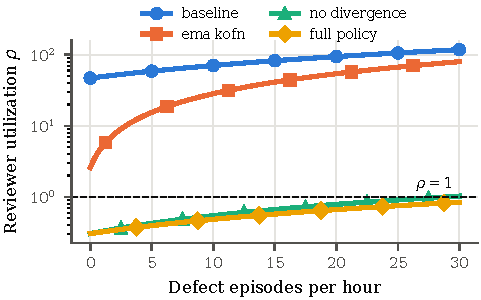
\includegraphics[width=\columnwidth]{operator_load.pdf}
\caption{Modeled utilization of one reviewer (assumed $\mu = \MuReviews$ reviews/h) as a function of the defect-episode rate, using the measured alerts per episode, alerts per glare burst (assuming \GlareRateAssumed{} bursts/h) and nominal false-alert rate of each policy (independent frame scores). Values above $\rho = 1$ mean an unbounded backlog under an $M/M/1$ model.}
\label{fig:load}
\end{figure}

\subsection{Operator load}
\label{sec:load}
The workloads compress many events into five minutes, so their hourly alert rates overstate a real line. Fig.~\ref{fig:load} combines the per-event measurements with two \emph{assumed} rates: \GlareRateAssumed{} glare bursts per hour and $\mu = \MuReviews$ reviews per hour. Under an $M/M/1$ model~\cite{shortle2018fundamentals}, one reviewer is overloaded by the baseline even without defects and by \texttt{EMA\_KOFN} because of glare alone. The full policy stays below $\rho = 1$ up to about \LoadCrossFull{} defect episodes per hour, the delay-timer up to about \LoadCrossTimer{} and decision fusion up to about \LoadCrossFusion{}, because the two baselines raise almost no glare alerts; on this metric the simple baselines are better. This is a model of utilization, not an observation of operators; the queue model assumes Poisson arrivals, whereas alerts are burstier, and operators also discount unreliable alarms~\cite{bliss1995trust,wickens2009false}.

\begin{figure*}[!t]
\centering
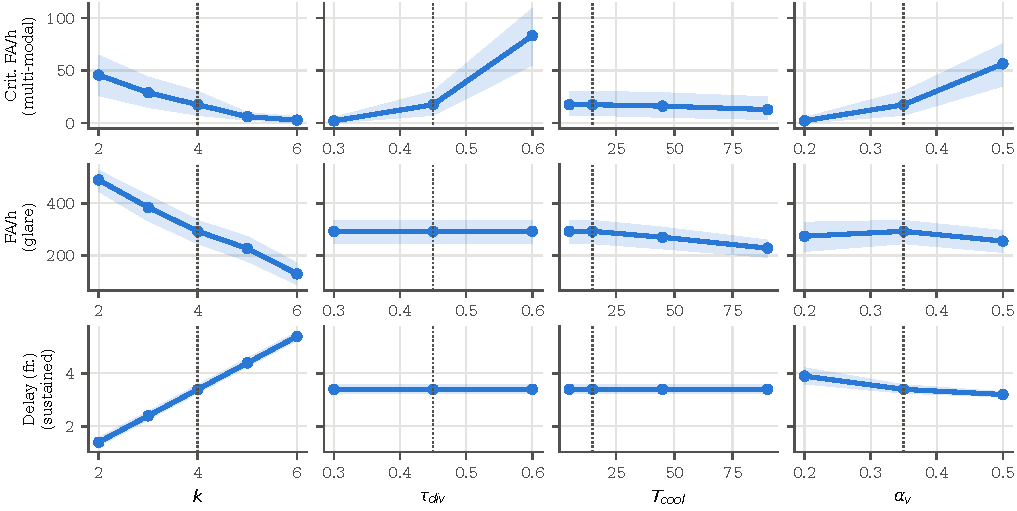
\includegraphics[width=0.9\textwidth]{sensitivity.pdf}
\caption{One-at-a-time sensitivity of the full policy (mean and 95\% bootstrap band over \UnitsPerCell{} units; dotted line: fixed default). Rows: false critical alerts per hour (multi-modal workload), false alerts per hour (glare workload), mean detection delay (sustained defects).}
\label{fig:sens}
\end{figure*}

\subsection{Sensitivity}
Fig.~\ref{fig:sens} varies one parameter at a time. With the revised rule~(4), critical false escalations stayed between \SensCritMin{} and \SensCritMax{} per hour for every tested value of every parameter, so they no longer depend on $\tau_{\text{div}}$ or $\alpha_v$. The parameters mainly trade glare alerts against delay: raising $k$ from \SensKLow{} to \SensKHigh{} lowered false alerts in the glare workload from \SensGlareKLow{} to \SensGlareKHigh{} per hour while the mean delay grew from \SensDelayKLow{} to \SensDelayKHigh{} frames, and longer incidents ($T_{\text{cool}}$ up to 90 frames) lowered them from \SensGlareCoolLo{} to \SensGlareCoolHi{} per hour. Recall on the multi-modal workload never fell below \SensRecallMin{}. The bands in this figure resample units, not categories, and are therefore narrower than the category-level intervals above.

\subsection{Latency}
\begin{table*}[!t]
\centering
\caption{Per-cycle latency on the inspection thread, paced at 30 frames/s (\LatCycles{} GPU and \LatCpuCycles{} CPU cycles per configuration; \LatNativeRes{} PNG frames; memory bank \MemoryBankSize{} patches). Synchronous: spool and audit inserts on the inspection thread. Writer thread: the inspection thread only enqueues the decision.}
\label{tab:latency}
\footnotesize\setlength{\tabcolsep}{4pt}
\begin{tabular}{@{}lrrrrr@{}}
\toprule
 & \multicolumn{3}{c}{GPU} & \multicolumn{2}{c}{CPU} \\
\cmidrule(lr){2-4}\cmidrule(lr){5-6}
Stage (ms) & mean & p99 & max & mean & p99 \\
\midrule
PNG decode & 10.06 & 13.05 & 23.8 & 10.99 & 14.13 \\
Optical check + PatchCore & 13.59 & 16.53 & 31.2 & 51.41 & 73.07 \\
Sensor step & 0.11 & 0.22 & 0.4 & 0.12 & 0.30 \\
Policy & 0.06 & 0.15 & 0.4 & 0.07 & 0.18 \\
Spool insert & 0.32 & 0.55 & 27.0 & 0.31 & 0.59 \\
Audit insert & 0.22 & 4.84 & 28.5 & 0.23 & 2.45 \\
\midrule
End to end & 24.36 & 36.06 & 55.6 & 63.12 & 88.76 \\
\bottomrule
\end{tabular}

\end{table*}
Table~\ref{tab:latency} times every stage with a real PatchCore forward pass on an \LatGpuName{}. With synchronous persistence the mean cycle took \LatGpuSyncMean{}\,ms (p99 \LatGpuSyncPNinetyNine{}\,ms) and \LatGpuSyncMiss{} of cycles exceeded the 33.3\,ms frame budget; single spool and audit inserts occasionally took up to \LatSpoolMax{} and \LatAuditMax{}\,ms. With the writer thread, enqueuing took at most \LatPersistMax{}\,ms, the mean cycle took \LatGpuAsyncMean{}\,ms (p99 \LatGpuAsyncPNinetyNine{}\,ms), and \LatGpuAsyncMiss{} of cycles missed the budget. The worst cycle did not improve (\LatGpuSyncMax{} vs.\ \LatGpuAsyncMax{}\,ms): the remaining misses come from PNG decoding (up to \LatDecodeMax{}\,ms) and the vision stage (up to \LatVisionMax{}\,ms). The price is durability: a decision reached disk at most \WriterLagMax{}\,ms after it was enqueued (p99 \WriterLagPNinetyNine{}\,ms; the writer queue never held more than \WriterMaxDepth{} pending decision), and would be lost in a crash within that window. Neither configuration is hard real-time. On the CPU alone the cycle took \LatCpuAsyncMean{}\,ms with the writer thread and missed the budget in \LatCpuAsyncMiss{} of cycles. On embedded hardware, the companion study~\cite{sengar2026paperB} compiled the same ResNet-18 PatchCore scoring path to TensorRT~10.16 in FP16 on a Jetson Orin Nano (15\,W mode): paced at 30\,FPS, the scoring pipeline took a median of 8.2\,ms per frame (p95 8.6\,ms) including host--device copies, reached 243\,FPS unpaced, and the module drew 3.98\,W (0.85\,W above idle), with decisions identical to FP32 on its test frames.

\subsection{Durable delivery}
\begin{table}[!t]
\centering
\caption{Delivery through a real Mosquitto \SpoolBrokerVersion{} broker at 30 events/s (QoS 1, synchronous spool inserts). Miss.: events never received; Evict.: removed by the spool capacity; Dup.: repeated deliveries; Order: first deliveries out of sequence; Peak: largest spool depth.}
\label{tab:durability}
\footnotesize\setlength{\tabcolsep}{3.5pt}
\resizebox{\columnwidth}{!}{\begin{tabular}{@{}lrrrrrrr@{}}
\toprule
Fault & Events & Miss. & Evict. & Dup. & Order & Peak & Drain (s) \\
\midrule
Link loss 30\,s & 1{,}051 & 0 & 0 & 0 & 0 & 901 & 1.85 \\
Link loss 60\,s & 1{,}951 & 0 & 0 & 0 & 0 & 1{,}801 & 1.22 \\
Link loss 120\,s & 3{,}751 & 0 & 0 & 0 & 0 & 3{,}601 & 1.97 \\
Broker restart 30\,s & 1{,}051 & 0 & 0 & 0 & 0 & 901 & 1.67 \\
Publisher SIGKILL & 600 & 0 & 0 & 0 & 0 & 440 & 1.65 \\
Overflow (cap.\ 1{,}000) & 1{,}951 & 802 & 802 & 0 & 0 & 1{,}000 & 0.56 \\
\bottomrule
\end{tabular}
}
\end{table}
Table~\ref{tab:durability} reports six fault cases. Link losses of up to \SpoolMaxOutage{}\,s (\SpoolMaxEvents{} events), a broker restart and a SIGKILL of the publisher during draining lost no event, delivered none out of order, and drained within \SpoolMaxDrain{}\,s after recovery. When a 60\,s outage exceeded a 1{,}000-record spool, the spool evicted \SpoolOverflowEvicted{} events and \SpoolOverflowMissing{} were missing, so every loss was accounted for (\SpoolUnexplainedMissing{} unexplained). Because the spool counts but does not record evicted identifiers, an evicted event that had already been sent could still arrive; this happened \SpoolOverflowEvictedDelivered{} times in this run. The crash run produced \SpoolCrashDuplicates{} duplicates; duplicates are possible by design and are removed by identifier. These tests cover the publisher and broker; we did not test subscriber crashes, power loss or exactly-once processing.

\subsection{Synthetic sensor traces}
\begin{table}[!t]
\centering
\caption{Replay of two synthetic run-to-failure traces (600 frames, shape inspired by the IMS bearing~\cite{qiu2006wavelet} and C-MAPSS~\cite{saxena2008damage} data but not derived from them) with good-part visual scores, means over the seven categories. First flag: first non-normal decision relative to the labeled onset (negative = before). Alerts before/from the onset.}
\label{tab:trace}
\footnotesize\setlength{\tabcolsep}{3.5pt}
\resizebox{\columnwidth}{!}{\begin{tabular}{@{}llrrr@{}}
\toprule
Trace & Policy & pre-fault FA/h & recall & delay (fr.) \\
\midrule
Bearing proxy & \texttt{BASELINE} & 4{,}243 & 0.43 & 8.3 \\
 & \texttt{NO\_FUSION} & 0 & 0.00 & -- \\
 & \texttt{FULL\_POLICY} & 300 & 1.00 & 0.0 \\
\midrule
Thermal-creep proxy & \texttt{BASELINE} & 4{,}208 & 0.57 & 3.5 \\
 & \texttt{NO\_FUSION} & 0 & 0.00 & -- \\
 & \texttt{FULL\_POLICY} & 327 & 1.00 & 0.0 \\
\bottomrule
\end{tabular}
}
\end{table}
Table~\ref{tab:trace} checks the sensor path in isolation. The full policy first flagged both traces \TraceFirstFlagFullMin{}--\TraceFirstFlagFullMax{} frames \emph{before} the labeled onset, during the incipient drift, with a single \textsc{Review} alert; it raised no further alert and no \textsc{High} alert after the onset, because rule~(5) routes sensor-only evidence to review. Whether that early review counts as a timely detection or a false alert depends on where the fault is said to begin. A vision-only policy cannot see these faults; the baseline's alerts are chance crossings of nominal scores.

\section{Threats to Validity}
\emph{Data.} All visual scores come from \NumCategories{} curated MVTec AD categories with small good-image pools. With the same ResNet-18 PatchCore at the 99th-percentile threshold, the companion study~\cite{sengar2026paperB} measured a median per-image recall of 0.94 on MVTec AD but 0.57 on the 12 VisA~\cite{zou2022visa} categories and 0.72 on VisA at $448\times448$ input. The policy can delay or merge detections but not create them, so such detector losses carry over to the alert stream.
\emph{Temporal realism.} Scores are sampled from pools rather than taken from video; the correlated rerun shows that conclusions about false alerts on good parts depend strongly on this choice. Glare is synthetic, sensors are simulated and the traces are synthetic.
\emph{Workload density.} Event densities are much higher than on a real line, which is why Section~\ref{sec:load} models load per event; the load model uses assumed rates and is not an observation of operators.
\emph{Optical check.} The blur check misfired on real defects: in \OpticalWorstCategory{} it flagged \OpticalWorstRate{} of defective test images (\OpticalWorstTypes{}) as blurred, which would route those parts to a camera-maintenance review, while no good test image was flagged; the workloads run the check on good training frames and therefore do not exercise this failure.
\emph{Statistics.} Seven categories are few clusters; category-level intervals are wide, and per-category differences in Table~\ref{tab:effects} are often ties.
\emph{Post-hoc change.} Rule~(4) was revised after inspecting the first ablation; the external baselines were defined before they were run.
\emph{Systems.} Latency was measured on one laptop GPU without camera acquisition or network transport, and delivery guarantees are broker-level at-least-once only.

\section{Conclusion}
Wrapping a visual anomaly detector in alarm-management primitives is useful only in combination, and no single design dominated. The integrated policy gave the fewest false line-stop escalations, used sensors to see faults the camera cannot, and handled machine states and degraded inputs that simple alarms ignore; a plain delay-timer suppressed short glare far better at the cost of missing defects shorter than about half a second; and every persistence-based design lost its zero false-alert result once consecutive scores were correlated. Acknowledgment-driven spooling kept every event through the outages we tested, and a writer thread more than halved the frame-budget misses at the price of a small crash window, without removing the worst-case cycle. The most important open question is how these rankings change on real, temporally correlated inspection video. Code, configuration, scores and every generated table and figure are available at \url{https://github.com/sengarutk/edge-quality-intelligence}; \texttt{scripts/reproduce\_all\_paper\_results.sh} regenerates them.

\bibliographystyle{IEEEtran}
\bibliography{references}

\end{document}
